\chapter{Spin Glass}
\label{chap:SGintro}
\section{Introduction}
Spin glasses are magnetic systems where the frozen-in quenched structural 
disorder leads to conflicting magnetic moments, which prevents the formation 
of long range magnetic ordering, e.g.,ferromagnetic ordering.

The prototype material is a dilute magnetic alloy, with a small amount of 
magnetic impurity (such as Fe, Mn) randomly substituted into the lattice of a 
noble metallic host (i.e. Cu, Au). Insulators such as Eu$_x$Sr$_{1-x}$S, with $x$
between 0.1 and 0.5 also show spin glass behavior.
 
The physics underlying the spin glass behavior comes from the quenched 
randomness: a pair of spins have a roughly equal a priori probability of having
a ferromagnetic or an anti-ferromagnetic interaction. For the dilute magnetic 
alloy, the conduction electron-mediated 
Ruderman-Kittel-Kasuya-Yoshida (RKKY) interactions between the localized moments
 oscillates strongly with distance, 
 \begin{equation}
   \label{eq:RKKY}
   J(R)=J_0\frac{\cos(2k_FR+\phi_0)}{(k_FR)^3}, R\rightarrow 0
 \end{equation}
Here $J_0$ and $\phi_0$ are constants, and $k_F$ is the Fermi wave number of the
host metal. Since the distances between the spins are random, some of the $R$
will be positive, some will be negative,
thus forming ferromagnetic/anti-ferromagnetic bonds randomly, and no spin 
alignment would satisfactory all exchange bonds. 



\begin{figure}[!h]
  \label{fig:rkky}
  \centering
  \includegraphics[width=0.6\textwidth]{img/RKKY.png}
  \caption{Sketch of RKKY interaction.}
\end{figure}

Experiments demonstrated some unusual features of spin glass materials, 
including the cusp in the low-field, low-frequency susceptibility and the 
discrepancy of magnetic response between zero-field and field cooling 
measurements, as shown in Fig \ref{fig:experimentsSG}. These facts suggest that spin glass system has no conventional 
long range magnetic ordering and exhibits very slow dynamics. 

\begin{figure}[!h]
  \label{fig:experimentsSG}
  \centering
  \subfigure[Low frequency susceptibility of CuMn with 1\% Mn, (Mulder et al 1981)]
  {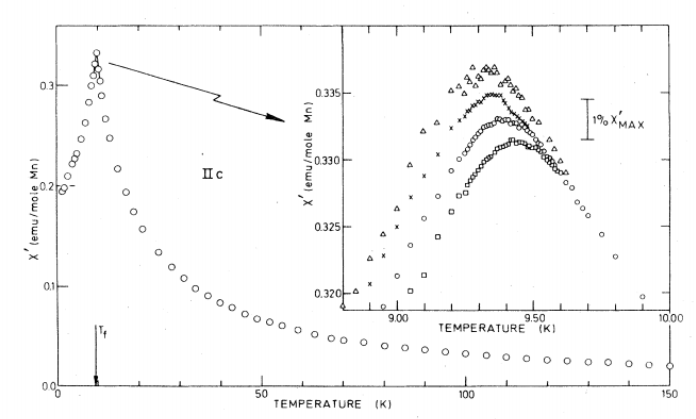
\includegraphics[width=0.6\textwidth]{img/cusp_low_freq.png}}\\  
\subfigure[Susceptibilities of CuMn vs temperature for 1.08\% and 2.02\% Mn.
(Natata et.al 1979)]
{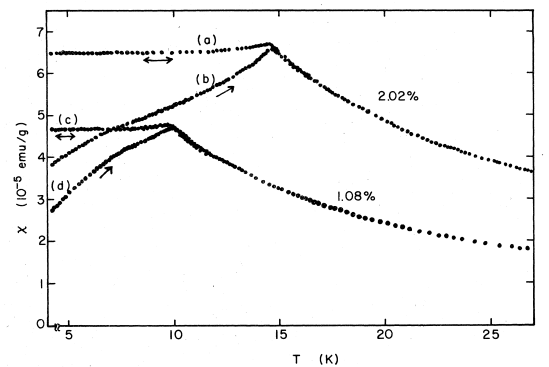
\includegraphics[width=0.6\textwidth]{img/fc_zfc.png}}
  \caption{Magnetic features of spin glass in a small field.}
\end{figure}

\section{Theoretical understanding on spin glass}
The simplest model that captures the consequences of disorder is an Ising model 
with quenched randomly disordered couplings, first proposed by Edwards and 
Anderson:
\begin{equation}
  \label{eq:EA}
  H=-\sum_{\langle i,j \rangle}J_{ij}S_iS_j-h\sum_iS_i
\end{equation}
Here $S_i$ is the spin in a $d$-dimensional lattice that can take values $\pm 1$,
$\langle i,j \rangle$ indicates nearest neighbors with the coupling $J_{ij}$ between 
them, and $h$ is the external field.
 
Two main paradigmatic cases for the $J_{ij}$ in EA model are:
\begin{itemize}
\item Gaussian distribution of random coupling:
  \begin{equation}
    \label{eq:Jij_Gaussian}
    P(J_{ij})=\frac{1}{\sqrt{2\pi}}\exp^{-J_{ij}^2/2}
  \end{equation}
\item Bimodal ($\pm J$) distribution of random coupling:
  \begin{equation}
    \label{eq:Jij_bimodal}
    P(J_{ij})=\frac{1}{2}[\delta(J_{ij}-1)+\delta(J_{ij}+1)]
  \end{equation}
\end{itemize}

\subsection{Frustration}
\label{sec:frustration}
Frustration may be present the Hamiltonian \ref{eq:EA} when no spin 
configurations can satisfy all couplings at the same time. 

\begin{figure}
  \centering
  \subfigure[Geometrical Frustration. Here all couplings are anti-ferromagnetic.]{
    \label{fig:frustration_geo}
    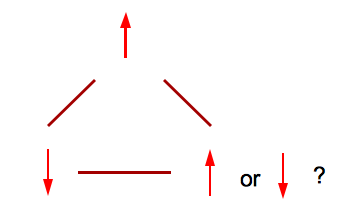
\includegraphics[width=0.4\textwidth]{img/ising-3-spin.png}
  }\hspace{0.5cm}
  \subfigure[Frustration due to randomness. Here $J=-1$ indicates an 
anti-ferromagnetic coupling, while $J=+1$ means ferromagnetic coupling.]{
    \label{fig:frustration_quench}
    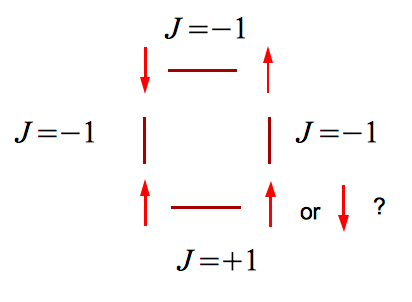
\includegraphics[width=0.4\textwidth]{img/ea-4-spin.png}
  }
  \caption{Frustration in EA model.}
  \label{fig:frustration}
\end{figure}

Figure \ref{fig:frustration} demonstrate two situations where frustrations 
happens. In Fig \ref{fig:frustration_geo}, the two spin on the top and the left
are anti-parallelly aligned due to the anti-ferromagnetic coupling between them,
but there is not an preferred spin direction for the third spin that can satisfy
both the anti-ferromagnetic bonds. In Fig \ref{fig:frustration_quench}, the 
frustration comes from the random distribution of $J_{ij}$. 

\subsection{Mean Field Model}
\label{sec:meanfield-model}

An infinite-ranged version was proposed by Sherrington and Kirkpatrick (SK).
\begin{equation}
  \label{eq:SK}
  H=-\frac{1}{\sqrt{N}}\sum_{1\le i\le j\le N}J_{ij}S_iS_j
\end{equation}
Here $J_{ij}$ is chosen from a Gaussian distribution in equation 
\ref{eq:Jij_Gaussian}.

This model has an equilibrium phase transition at $T_c = 1$.
For the spin glass phase below $T_c$, Parisi employed a novel ansatz and 
developed a  possible physical interpretation of the nature of spin glass, 
which is now known as the ``Replica Symmetry Breaking'' (RSB) picture. The main
idea behind the picture is that the spin glass phase consists of an infinite 
number of ``pure states'' that form a hierarchy rather than follow simple symmetry
transformation. 

A competing picture, known as droplet/scaling, is based on domain-wall 
renormalization group ideas. In this picture, there is only a single of
pure states that are spin-flip-symmetrical at low temperature in any finite 
dimension. 


\section{Quantities characterizing spin glass}
The quantity $q$ measures the breaking of time-reversal symmetry, and is now 
known as the ‘EA order parameter’.
\begin{equation}
  \label{eq:q}
  q=\frac{1}{N}\sum_iS_i^\alpha S_i^\beta
\end{equation}
where $\alpha$ and $\beta$ are two copies of lattice with the same disorder 
configuration, but simulated with different random seeds, so they are
statistically independent of each other. 

According to the Parisi solution, for fixed J and (large) N, the structure of 
the overlap is nontrivial.

\section{Computer simulations review}

Universality in three-dimensional Ising spin glasses: A Monte Carlo study
arXiv:cond-mat/0602212 Phys. Rev. B, 73, 224432 (2006)



\section{Outstanding problems}
%• Is there a phase transition to a low-temperature spin glass phase?

• Are there infinitely many pure state pairs below Tc in the EA spin glass?

• If there do exist infinitely many equilibrium states in some finite 
dimensions, is their organization similar to that of the Parisi solution of the 
SK model?


\section{Difficulties}
The EA model is a deceptively simple problem. %Since it is a classical spin 
%model, one may think that its numerical study can be simply carried out by Monte
%Carlo methods on conventional hardware. 
One of the defining signatures of spin glass systems is their long relaxation 
time. 
For sufficiently low temperatures, the system becomes very sluggish and 
equilibration is prohibitively difficult even for modest systems sizes. 
Moreover, it has been shown that finding the ground state of the three 
dimensional EA model is an NP-hard problem. \cite{Barahona-1982} 
Until recently, there has been no consensus on whether there is a finite spin 
glass critical temperature in the three dimensional EA model.

It also requires a large number of disorder realizations to reach any 
meaningful result.


\section{Algorithms for spin glass simulation}
The breakthrough in the numerical study of spin glass systems came with the 
introduction of the parallel tempering method.

Simulated annealing (SA) is a method for solving unconstrained and 
bound-constrained optimization problems.

Population annealing combines simulated annealing and Boltzmann weighted 
differential reproduction within a population of replicas to sample equilibrium 
states.

Another possibly to overcome the diverging autocorrelation time problem is the 
multicanonical reweighting method.

%%% Local Variables:
%%% mode: latex
%%% TeX-master: "../thesis"
%%% End:
